\documentclass[]{article}
\usepackage{hyperref,geometry,fancyhdr,graphicx,needspace}
\usepackage{titlesec,xcolor}
\usepackage{baskervald}
\usepackage{setspace}\setstretch{1.05}

\geometry{width=5.5in,height=8.5in,centering}

\setlength{\parskip}{4pt}
\setlength{\parindent}{14pt}


% have running title and page number
\fancyhead{}\fancyfoot{}
\newcommand*{\topic}{Scientific Inference}
\fancyfoot[l]{\small\sc Understanding Science}
\fancyfoot[C]{\small\sc page \thepage\ of \pageref{theend}}
\fancyfoot[R]{\small\sc\topic}
\renewcommand*{\headrulewidth}{0pt}
\renewcommand*{\footrulewidth}{0pt}


\hypersetup{pdftitle={Understanding Science}, pdfauthor={P.D. Magnus}, pdfborder = {0 0 0 0}}

\newcommand*{\newbit}{\paragraph{\P}}

\newcommand*{\therefore}{${_\circ}$\hspace{-2pt}${^\circ}$\hspace{-2pt}${_\circ}$}

%\renewcommand*{\thesection}{\Roman{section}}
%\renewcommand*{\thesubsection}{\Alph{subsection}}
\renewcommand*{\thesection}{\Alph{section}}
\renewcommand*{\thesubsection}{$\bullet$}
\renewcommand*{\thesubsubsection}{$\circ$}
\setcounter{tocdepth}{2}


% The {earg} environment is used for arguments and example sentences.
\newcounter{eargline}
\newcounter{OLDeargline}
\newcounter{earginstance}
% EARGLIST
\newenvironment{earglist}[1]%
{%
\bigskip
\begin{minipage}{\textwidth}
\noindent%
\setlength{\unitlength}{12pt}%
\begin{picture}(5,1)%
\put(-.5,1){\line(1,0){5}}%
\put(-.5,0){\line(0,1){1}}%
\end{picture}%
\vspace{-14pt}\\%
\textsf{#1}%
\vspace{-6pt}%
\begin{list}{\arabic{eargline}.}{\usecounter{eargline}\setlength{\itemsep}{-.4em}}%
}%
{%
\setcounter{OLDeargline}{\arabic{eargline}}\end{list}%
\vspace{-6pt}%
\begin{picture}(5,1)%
\put(-.5,1){\line(1,0){5}}%
\put(-.5,1){\line(0,1){1}}%
\end{picture}%
\end{minipage}
}
% EARG
\newenvironment{earg}%
{\refstepcounter{earginstance}\begin{earglist}{Argument \#\arabic{earginstance}}}%
{\end{earglist}}
% Used in conjunction with {earg}, this handles the numbering and
% references to example sentences:
\newcounter{Example}%[chapter]
\newcommand*{\ex}[1]{\refstepcounter{Example}\arabic{Example}.\label{#1}}


\newcommand*{\terminology}{\paragraph{A point about terminology:}}


\begin{document}
\pagestyle{fancy}

\section*{Understanding Science: Scientific Inference}

\renewcommand{\contentsname}{\vspace{-48pt}}
\setcounter{tocdepth}{1}
\tableofcontents



\newbit This document is \copyright 2017--21 by P.D. Magnus. Some rights reserved.

It is offered under a Creative Commons Attribution 4.0 license.
You are free to copy this book, to distribute it, to display it, and to make derivative works, under the condition of Attribution. You must give the original author credit. This complete and precise license is available on-line at \url{http://creativecommons.org/licenses/by/4.0/}

This document is current as of \today






\newpage

% Create some nice looking section dividers without too much fuss
\titleformat\section{\Large\bf}{}{0 em}
  {%
  	\needspace{48pt}
    \begingroup
      \color{gray!30}%
      \titleline{\leaders\hrule height 0.2 em\hfill\kern 0 pt\relax}%
      \titleline{\leaders\hrule height 0.2 em\hfill\kern 0 pt\relax}%
    \endgroup
    \nobreak
    \center
    Section \thesection:~
  }

\titleformat\subsection{\large\it}{}{0 em}
  {%
  	\needspace{36pt}
    \begingroup
      \color{gray!30}%
      \titleline{\leaders\hrule height 0.2 em\hfill\kern 0 pt\relax}%
    \endgroup
    \nobreak
    \center
  }





%: INFERENCE
\section{Arguments}


An \emph{argument} is supposed to give you reasons to believe something. It has \emph{premises}, which are claims that you are asked to accept at the outset. They can be things that you already believe, or they may be things that were established by other arguments. An argument also has a \emph{conclusion}, which is the claim to which the argument leads you. Given that you accept the premises, the argument is supposed to provide you reason to believe the conclusion.

When people mean to give arguments, they typically often use words like `therefore' and `because.' Yet they do not necessarily put the premises at the beginning and the conclusion at the end. When analyzing an argument, the first thing to do is to separate the premises from the conclusion. Words like these are a clue to what the argument is supposed to be, especially if the conclusion comes at the beginning or in the middle of a paragraph.

\begin{description}
\item[premise indicators:] because, as, for, since, given that
\item[conclusion indicators:] therefore, hence, thus, then, so, consequently, it follows that, as a result, we may infer that, this implies that
\end{description}
%could expand this list

In order to make it clearer, we will typically present an argument as a list of sentences, putting the premises at the beginning and the conclusion at the end. We mark the conclusion with the symbol `\therefore', which abbreviates the word `therefore'.

\newbit
In general, there are two ways to answer or attack an argument. First, you can challenge the premises. An argument only gives you a reason to believe the conclusion \emph{if} you believe the premises, so denying the premises gives you space to reject the conclusion. Second, you can challenge the connection between the premises and the conclusion. That connection can be different for different kinds of argument.

\paragraph{A note to the reader:} This chapter uses numerous sample arguments to introduce various logical concepts. You should read the sample arguments and think for yourself: `Is this the sort of thing that I would accept as a reason?'

\subsection{Deduction}

Consider this classic example of an argument:

%\begin{earg}
%\item All men are mortal.
%\item Socrates is a man.
%\item[\therefore] Socrates mortal.
%\end{earg}



\begin{earg}
\label{all-are-mortal}
\item All humans are mortal.
\item All philosophers are human.
\item[\therefore] All philosophers are mortal.
\end{earg}

Given the argument, should you believe that all philosophers are mortal?

Probably, but perhaps you doubt one of the premises. You might wonder whether there are some non-human philosophers, perhaps in outer space. Alternately, you might think that some humans are not mortal.

If you accept the premises, however, there is no other room for doubting the conclusion. If the premises are true, then the conclusion must be true. This is because of the \emph{form} of the argument. Any argument with the same form is just as strong.

Consider this one:

\begin{earg}
\label{mizensporks}
\item All mizensporks are ghosby.
\item All eldreds are mizensporks.
\item[\therefore] All eldreds are ghosby.
\end{earg}

Here, it is unclear whether you ought to believe the premises. You do not even know what all those words mean! Yet this has the same form as \#\ref{all-are-mortal}. If the premises are true, then so is the conclusion. Schematically, the pattern is:

\begin{earglist}{The general form}
\item All Bs are Cs.
\item All As are Bs.
\item[\therefore] All As are Cs.
\end{earglist}

With an argument like this, it is impossible for the premises to be true and the conclusion false. This makes it \emph{deductively valid} or just \emph{valid}. An argument which is not like this, where it is possible for the premises to be true with the conclusion false, is called \emph{invalid}.

Note that knowing that an argument is valid does not tell you whether the premises or the conclusion are \emph{actually} true or false.

Consider this example:

\begin{earg}
\label{saxophones}
\item All electrical things are rosy.
\item All saxophones are electrical.
\item[\therefore] All saxophones are rosy.
\end{earg}

This argument has the same form as \#\ref{all-are-mortal} and \#\ref{mizensporks}. Since that form is valid, this argument is also valid. Yet the premises are obviously false. A valid argument which has one or more false premises might have a true conclusion, but it might (like this one) have a false conclusion. If the premises are false, then the argument gives you no reason to believe the conclusion.

\newbit A deductively valid argument is just defined as an argument where \emph{it is impossible for the premises to be true and the conclusion false}. It is worth saying a bit more about what counts as `impossible'.

For a deductively valid argument, there is no logical possibility of the conclusion being false if the premises are true. This holds even in the wildest possible world you can imagine, a crazy world where the laws of physics are different or where magical forces make everything wild and trippy.

There are other senses of possibility and impossibility which are not relevant. For example, because of the laws of physics, it is physically impossible for something to go faster than the speed of light. Even if there is no way around the laws of physics, there is no contradiction in considering something going faster than the speed of light. So something going faster is logically possible.

Consider \#\ref{all-are-mortal} and imagine that the conclusion were false, that there were some immortal philosopher. We can consider such a situation and reason about it, so it is logically possible even though it is medically and even perhaps physically impossible. Imagining the conclusion to be false, we realize that one or both of the premises must be also false. In a crazy world of undying highlander philosophers, either those philosophers would not be human (and so premise 2 would be false) or they would be counterexamples to the claim that all humans are mortal (and so premise 1 would be false).

There are deep philosophical puzzles here, but it is enough for our purposes to note that the `impossibility' in the definition of validity is \emph{logical impossibility}.

\terminology In ordinary conversation, the word `valid' has other meanings. If someone raises a concern, you might say, ``That's a valid point.'' But philosophers tend to just use the word `valid' when talking about deductive validity. So, when talking with philosophers, it is clearer just to use `valid' in the narrower sense. What you might ordinarily call a valid concern can be unambiguously called `genuine' or `legitimate'.

\paragraph{Exercise:} Give an example of a valid argument with false premises but a true conclusion.


\subsection{Ampliative inference}

Not all arguments are deductive, and validity is simply too strong a standard for arguments which are not meant to be deductive.

Consider this argument:

\begin{earg}
\item Most comic books are about superheroes.
\item Jen likes to read comic books.
\item[\therefore] Jen likes superheroes.
\end{earg}

This does not seem like a terrible argument. If you knew the premises to be true, then you would have a reason to believe the conclusion. Given that Jen likes comics, it would be reasonable to think that Jen probably likes superheroes. Yet she might just like comic books that do not have superheroes in them, or she might read superhero comics only because she likes the background illustrations.

Since it is possible for the conclusion to be false even if the premises are true, the argument is \emph{invalid}. If we evaluate it as a deductive argument, the only question is whether it is valid or not--- and this argument is not valid.

Yet it seems unfair to evaluate this as a deductive argument. Imagine someone says that they think Jen likes superheroes, you ask them why, and they provide these premises as reasons. It does seem relevant at least, and it does provide some evidence. This argument gives reasons for the conclusion, even though the reasons are not utterly decisive.

Instead of stating just a necessary consequence of the premises, the conclusion of the argument `goes beyond' the premises in a way. Arguments like this are called \emph{ampliative arguments}, because they add to or amplify what is already known and given in the premises.

We make ampliative arguments all the time, when we infer things which are not strict, deductive consequences of what we observe and what we know. Consider another example:

\begin{earg}
\item I am expecting my ride any time now.
\item They probably will not actually get out of the car when they get here.
\item I hear the honk of a car horn from in front of my house.
\item[\therefore] My ride is here.
\end{earg}

I am sufficiently confident of the conclusion that I grab my things and head out the door without enumerating the premises and spelling out the conclusion in this way. So the argument seems like a pretty strong one. Yet it is not valid. Perhaps the honking is some different car and not my ride at all. Perhaps it is an errant goose doing the honking.

For deductive arguments, there are just two possibilities: they can be either valid or invalid. For ampliative arguments, they can be \emph{strong} or \emph{weak} in varying degrees. The inference about my ride seems fairly strong, the inference about Jen liking superheroes seems less strong. 

\terminology Philosophers often call ampliative arguments \emph{inductive}, which makes an explicit contrast between deduction (where the good arguments are valid) and induction (where the good arguments are strong but strictly speaking invalid). However, as we will see, the word `induction' is also used in a narrower sense to indicate reasoning which generalizes from past experience.

\section{Enumerative induction}

There is a common kind of ampliative inference which appeals to a sample of observed instances and generalizes to unobserved instances. This often means appealing a historical track record and concluding that what held for those cases both held for other past cases and will hold for future cases.

For example:

\begin{earg}
\label{25-inches}
\item In 1965, there was more than 25 inches of precipitation in Albany.
\item In 1966, there was more than 25 inches of precipitation in Albany.
\item[] \ldots and so on, for the years in between\ldots
\addtocounter{eargline}{43}
\item In 2010, there was more than 25 inches of precipitation in Albany.
\item In 2011, there was more than 25 inches of precipitation in Albany.
\item[\therefore] Every year, there is more than 25 inches of precipitation in Albany.
\end{earg}

This form of argument is called \emph{enumerative induction}, because it enumerates many specific instances and generalizes to draw a conclusion about other instances.

The premises are about cases that are similar in some respect: here, they are specific years of precipitation in Albany. The conclusion is about all such cases: every year.

We do make such inferences, and sometimes we count them as strong.

Regardless of how strong you might think this argument is, it is not deductively valid. It is easy to imagine a year with less than 25 inches of precipitation, so it is at least logically possible that there were or will be such years. Moreover, the conclusion is actually false. In 1964, there was 21.55 inches of precipitation in Albany. That is the lowest level, going as far back as we have records.

In order to strengthen the argument, then, we might enlarge the evidence base and weaken the conclusion somewhat. So consider this alternative argument:

\begin{earg}
\item In every year for which we have records, there was more than 21 inches of precipitation in Albany.
%\item In 1826, there was more than 21 inches of precipitation in Albany.
%\item In 1827, there was more than 21 inches of precipitation in Albany.
%\item[] \ldots and so on, for the years in between\ldots
%\addtocounter{eargline}{183}
%\item In 2011, there was more than 21 inches of precipitation in Albany.
\item[\therefore] Every year, there was or will be more than 21 inches of precipitation in Albany.
\end{earg}

This includes more evidence and draws a more conservative conclusion than \#\ref{25-inches}, so it is clearly a stronger argument. Yet it is still not deductively valid.

One might worry about drawing a conclusion about \emph{every year}. The climate was different in the distant past and it will be different in the future. So one might make the argument even more cautious:

\begin{earg}
\label{21-inches-next-year}
\item In every year up until now, there was more than 21 inches of precipitation in Albany.
%\item In 1826, there was more than 21 inches of precipitation in Albany.
%\item[] \ldots and so on, for the years through 2011\ldots
\item[\therefore] Next year, there will be more than 21 inches of precipitation in Albany.
\end{earg}

Even this is not deductively valid. We can imagine that next year will be a drought worse than the one in 1964, even if no such drought actually occurs.

Yet \#\ref{21-inches-next-year} seems to be a strong argument. Even though we do think that climate is changing, we still expect next year's weather to be more or less like that long run of weather from the last couple of centuries. Farmers and gardeners plant crops with the expectation that there will be roughly the usual amount of rain. They do this on the basis of experience, relying implicitly on something like \#\ref{21-inches-next-year}. Even though it is not a deductively valid inference, we don't think of farmers as being irrational.

However, we may wonder what it is that makes inductive inference legitimate.

\subsection{Hume's problem}

The eighteenth-century Scottish philosopher David Hume famously asked what justifies our learning from experience. His answer was that there is no rational justification for induction.

He begins by asking what sort of justification we could possibly have.

It is not the case that the premises of \#\ref{21-inches-next-year} make the conclusion necessary, because it is not a deductively valid argument. It is does not follow just as a matter of logic that next year will be like the other years on record.

Surely, though, we have learned from experience that weather tends to be in certain ranges. We talk about climate because we think that even though weather does vary from year to year, there are general regularities and patterns.

Some philosophers have thought that enumerative induction relies on a general principle that the future will resemble the past. That is to say, we know that nature is uniform. Let's call this the \emph{Principle of the Uniformity of Nature} or PUN. If we add PUN as a premise to \#\ref{21-inches-next-year}, then it becomes a different argument.

\begin{earg}
\label{21-inches-PUN}
\item In every year up until now, there was more than 21 inches of precipitation in Albany.%\item In 1826, there was more than 21 inches of precipitation in Albany.
%\item[] \ldots and so on, for the years through 2011\ldots
%\addtocounter{eargline}{184}
%\item In 2011, there was more than 21 inches of precipitation in Albany.
\item What was true of all those past years will be true of next year.
\item[\therefore] Next year, there will be more than 21 inches of precipitation in Albany.
\end{earg}

Here we have added PUN as premise 2. Note that this makes the argument deductively valid. Think about that for a minute. \emph{If} something were true of those past years \emph{and} next year must be like the past years, \emph{then} the same thing will be true of next year.

So relying on some version of PUN would give us an answer as to why enumerative inductions are good arguments. Just as farmers expect a certain amount of rain next year without explicitly writing down \#\ref{21-inches-next-year}, we could say that anyone who writes down \#\ref{21-inches-next-year} really has \#\ref{21-inches-PUN} in mind. Deduction is rational, and the idea here is to try and show that induction is rational by making it turn out to be implicitly deductive. All that is required is supplying an extra premise which is strong enough to make the argument valid.

Appealing to PUN in this way seems to give us an answer to the question of why arguments like \#\ref{21-inches-next-year} seem like good ones.

Hume would ask, however, why we believe the extra premise. How do we know that weather is regular in this way? In general, how do we know that nature is uniform?

It is logically possible that PUN itself could have been false, even if it has turned out to be true. We can imagine a world where the weather changes randomly from year to year, where past performance would be no guide to future results. There would be no climate to speak of in such a world. Creatures like us could not even survive there, because we rely on regularities to eat, move around, and avoid mortal peril.

So it seems as if PUN must be something we have learned from experience. But Hume's question at the outset was what could possibly \emph{justify} learning from experience.

Consider the enumerative induction which summarizes all of the past occasions when nature has turned out to be uniform, those times in which it was possible to learn from experience. It would look something like this:

\begin{earg}
\label{trackrecord-PUN}
\item Nature was uniform in every year up until now.
\item[\therefore] Nature will be uniform next year.
\end{earg}

It is unclear \emph{why} we should accept this argument. Just as we can imagine a topsy-turvy world in which it was never possible to learn from experience, we can imagine a world which has been regular just as ours has been but which becomes topsy-turvy next year. We would perish in the chaos, so we hope we are not in such a world. Moreover, we do not seriously worry about incoherent chaos erupting and the order of nature failing. But that is just to say we do accept something like \#\ref{trackrecord-PUN}. Hume's question is what justifies that acceptance.

The suggestion we were considering was that arguments like \#\ref{trackrecord-PUN} are justified by having PUN as an implicit premise. Writing it down explicitly, the argument becomes this:

\begin{earg}
\label{circular-PUN}
\item Nature was uniform in every year up until now.
\item \emph{What was true of all those past years will be true of next year.}
\item[\therefore] Nature will be uniform next year.
\end{earg}

The problem is that we must already know premise 2 in order to make use of this argument. Yet that premise is just that every coming year will be like the prior ones. If we already knew that, we would not need to collect the evidence expressed in premise 1.

So \#\ref{circular-PUN} presumes the very point which we were trying to establish. It cannot give us any new reason for believing its conclusion.

This is called a \emph{circular argument}, because it is justifies a claim on the basis of essentially that same claim. Instead of leading to some new conclusion, it leads from the premises right back to the premises.

So there does not seem to be any way to justify PUN, but without PUN there is no way to justify enumerative induction. So, Hume concludes, we do not have a justification for it. Nevertheless, we rely on induction throughout our lives.

Some philosophers have thought that we can rely on PUN without any justification. Like a mathematical axiom, it is something that we accept without having to give reasons for it. If that were correct, then PUN would be something that we are always entitled to as a premise but never need to establish as a conclusion. So \#\ref{trackrecord-PUN} and \#\ref{circular-PUN}, because they try to give reasons for PUN, would be deeply confused.

One problem is that this does not explain how PUN can be an axiom in this way. For Hume, something can only be unassailably true or axiomatic if it is true as a matter of definition. Yet the definition of `uniform' is not enough to guarantee that PUN is true. The fact that we can imagine an eruption of chaos where the uniformities break down shows that the falsity of PUN is at least conceivable.

Defenders of PUN might reply in different ways. This raises some tricky philosophical questions, but let's move on.

\terminology A circular argument is said to be \emph{question begging}. This is just what `begging a question' meant in its original sense: seeming to argue for a claim while really just assuming it. A circular or question begging argument cannot give you any reason to believe the claim that you didn't already have.

People now often use the phrase in a different way. Something `begs a question' in the new sense if it \emph{leads us to ask} the question. In order to avoid misunderstanding, it is best to avoid using the phrase in this latter way when talking about logic or philosophy.

\subsection{The historical Hume}

Many philosophers have thought that the only adequate answer to Hume's challenge was to somehow justify induction. Hume himself didn't think so.

He was writing before psychology became a discipline separate from philosophy, but part of what he was doing was what we now would call psychology. He was interested in figuring out how it is possible for us to learn from experience. For reasons we discussed in the last section, he thought that there is no \emph{justification} and so that induction could not be a matter of reason. Yet we do learn from experience nonetheless. How do we do it?

Hume's answer is that the mind works by forming cognitive habits. For example, when you see the sun rise every morning, you start to expect it. So you think that the sun will rise every morning.

Note that this does not show that you are \emph{justified}. Quite the contrary, Hume thinks that you do not have a reason for your expectation. Instead, he offers an explanation of how you form the belief by offering a psychological theory about how the human mind works. You form the expectation just because (to use a contemporary idiom) your brain is wired to form expectations.

Regardless, many philosophers have worried about whether induction can be justified. They do not just want to know \emph{how} we expect the future to be like the past, but \emph{why} we should believe it. This problem is typically called the \emph{problem of induction} or even sometimes \emph{Hume's problem} (even though Hume's own concern was with a slightly different problem).

\subsection{The new riddle of induction}

We have seen two responses to the problem of induction: According to one response, the Principle of the Uniformity of Nature (PUN) serves as an axiom that we rely on without justifying. According to Hume's response, though, we expect the future to resemble the past just because our brains are constructed in a way that makes us develop cognitive habits.

In the 20th-century, several philosophers showed that neither of these responses succeeds.

To take a famous example from Nelson Goodman, consider emeralds. All of the emeralds that anyone has ever seen are green. So we expect that any emeralds we find in the future will also be green.

According to the first response, this can be an explicit argument:

\begin{earg}
\label{all-green}
\item We have seen many emeralds, and all of those have been green.
\item PUN: Cases that have not been observed yet will resemble those that have already been observed.
\item[\therefore] All emeralds are green.
\end{earg}

According to Hume, we cannot make an explicit argument like this. Yet our minds work in a way so that after we have seen many green emeralds, we associate \emph{being an emerald} with \emph{being green}. And when we think of emeralds, we expect them to be green.

Goodman, though, asks us to imagine the category of \emph{grue} things. We define `grue' so that it includes anything which is green before the year 2020 and anything which is blue during or after that year. The specific year is not important; what matters is that we specify some point still in the future. The category of grue things includes all the emeralds that we have observed so far. All observed emeralds have been green, but (because of how we defined `grue') they have also all been grue.

The conclusion of \#\ref{all-green} is not just about emeralds we have observed, but about all the emeralds which we might ever observe. If all emeralds always really are green, then an emerald observed in the year 2021 will be green and not grue.

The problem comes when we consider this argument:

\begin{earg}
\label{all-grue}
\item We have seen many emeralds, and all of those have been grue.
\item PUN: Cases that have not been observed yet will resemble those that have already been observed.
\item[\therefore] All emeralds are grue.
\end{earg}

This has exactly the same form as \#\ref{all-green}. So, if the earlier argument is acceptable, then this one should be too.

Hume's approach leads us to a similar conclusion. On his account, our mind develops habits of expecting regularities to continue. Even though we wouldn't have put it this way before we learned the word `grue', we have seen many grue emeralds. So we should associate \emph{being an emerald} with \emph{being grue}.

However, we cannot accept the conclusion of both arguments! If all emeralds are green, then the ones observed in 2021 will not be grue. Conversely, if all emeralds are grue, then the ones observed in 2021 will not be green. It can't be the case that all emeralds are both green and grue.

The reasons for accepting one conclusion rather than the other are entirely symmetrical. Considering just the form of \#\ref{all-green} and \#\ref{all-grue}, both look like this:

\begin{earglist}{The general form}
\item We have seen many As, and all of those have been Bs.
\item PUN: Cases that have not been observed yet will resemble those that have already been observed.
\item[\therefore] All As are Bs.
\end{earglist}

Similarly for Hume, the mechanism of habit formation is formally the same in both cases. So there does not seem to be any reason to prefer one conclusion to the other, even though they cannot both be true.

Of course, people do prefer the first conclusion (in terms of green) over the second (in terms of grue). We are happy to think that green is a natural category and that grue is a philosopher's trick. Goodman's point is that appealing to PUN or habit formation cannot explain this difference.

This problem is typically called the \emph{new riddle of induction}, because neither of the answers to the original problem of induction can solve it.

Following Hume, we could just ask \emph{how} it is possible for us to do induction. The question is how we can think of emeralds as green but not grue when the considerations on each side appear to be the same. Goodman's answer is that we prefer to use \emph{entrenched predicates}. An entrenched predicate is just a term or category that we have used for a long time already. Green is entrenched, having a long history in English and in languages before it. Grue is not, because Goodman made it up. When we see many emeralds, it is true that they are both green and grue. We conclude that all emeralds are green because we have a long history of thinking in terms of `green'. This explains, as a psychological matter, how we can distinguish between the two conclusions.

Many philosophers find this unsatisfying. They want to know why we should conclude that emeralds are green but not that emeralds are grue, not just how we do. What justification do we have?

\newbit The new riddle underscores the difference between deductive and inductive arguments.

For deductive validity, only the form of the argument matters. Arguments \#\ref{all-are-mortal}, \#\ref{mizensporks}, and \#\ref{saxophones} all had the same general form. Because that form was valid, they were all valid arguments.

For inductive strength, form alone is not enough. Arguments \#\ref{all-green} and \#\ref{all-grue} have the same general form. Even if we were to change the second premise of each by rewriting PUN, the form of the arguments would still be same. Yet the inference from the first premise to the conclusion seems fairly strong in \#\ref{all-green} but terribly weak in \#\ref{all-grue}. 

Deductive validity is simply a matter of form, but inductive strength cannot be.


\newbit It is possible to pose the new riddle without introducing crazy terms like `grue'. More directly, we can point out all of the ways in which the future \emph{does not} resemble the past. Bertrand Russell gives the example of a chicken on a farm. It has been fed by the farmer every day, so it comes to expect only food from the farmer. Yet, as Russell says, ``The man who has fed the chicken every day throughout its life at last wrings its neck instead, showing that more refined views as to the uniformity of nature would have been useful to the chicken.''
%Domestic animals expect food when they see the person who feeds them. We know that all these rather crude expectations of uniformity are liable to be misleading. The man who has fed the chicken every day throughout its life at last wrings its neck instead, showing that more refined views as to the uniformity of nature would have been useful to the chicken.
%The Problems of Philosophy, Chapter VI, On Induction 

%To take another example: Through the end of the last century, the number of every year had been less than 2000. Yet nobody concluded, from the uniformity of nature, that all years forever would be less than 2000.

We think that the future will resemble the past in some respects, but there are many other respects in which we expect future instances to be different than cases we have observed so far. Our minds work so as to form some habits, expecting some regularities  to continue, but not to form others.

The new riddle is this: Why do we inductively generalize some patterns but not others? Why should we?


\subsection{The material theory of induction}

A modest answer to the problem of induction is to say that there is no general answer to it, but that we have specific background knowledge that allows us to get by in particular cases. For example, suppose we test two samples: one of a lump of pure gold, the other a plastic toy that I bought out of a vending machine. We melt them both, and find that the gold melts at $1064^{\circ}$C and the plastic at $164^{\circ}$C. We conclude that other samples of gold will melt at about the same temperature as this gold, but we don't draw a similar conclusion about plastic. Gold is an element, and there is only one kind of pure gold. Plastic is not, and there are many different kinds of plastic.

When we perform induction in this way, we rely on facts which we know about plastic and gold. When we make inductive inferences about the weather (like \#\ref{21-inches-next-year}) we rely on different background knowledge. There is no general principle of uniformity, which explains why philosophers have never been able to satisfactorily express PUN. Instead, there are disparate pieces of background knowledge which we rely on for different inductions.

Following the philosopher of science John Norton, let's calls this answer to the problem of induction \emph{the material theory of induction}. The bits of background knowledge which underwrite generalization in particular cases are \emph{material postulates}.

One might complain that the material theory of induction does not really solve the problem of induction. Although our knowing that gold is an element may explain why we generalize from this sample melting at about $1064^{\circ}$C to all samples having that melting point, this just introduces a regress: How do we know that gold is an element? How do we know that elements have stable melting points?





%: HD+IBE

\section{Inferring unobserved causes}

Imagine that I come home to see that my front window is shattered. When I unlock the door and go inside, I immediately notice that the television is not in the front room where it usually is. I yell to nobody in particular, ``I've been robbed!''

In the moment, I probably would not think of this inference as an explicit argument. If I did, it would look like this:

\begin{earg}
\label{robbed}
\item My window is broken.
\item My television is missing.
\item[\therefore] I've been robbed.
\end{earg}

This argument is not deductively valid. It is conceivable at least that the window shattered in a gust of freakishly strong wind and that television simply evaporated. So we should think of \#\ref{robbed} as an ampliative inference. We could disagree about how strong it is, but it is not especially weak. It is reasonable for me to think, seeing this evidence, that I have been robbed.

Something to note about \#\ref{robbed} is that it is not an enumerative induction. I do not observe a long history of robbers breaking windows and stealing televisions in order to infer some general fact about robberies.

Notice also that the concept of \emph{being robbed} appears in the conclusion of \#\ref{robbed} even though it does not appear in the premises. This does not happen in valid deductive arguments or enumerative inductions. In \#\ref{all-are-mortal}, for example, the conclusion can involve \emph{mortality} because the first premise assumes something about it. In \#\ref{25-inches}, the conclusion is about annual precipitation because the premises are all about annual precipitation.

The premises here are about things which I observe directly: The window is broken, and the television absent. The conclusion is about something which I do not directly observe, but instead propose as the explanation for why things are the way I observe them to be: A robber broke through the window and took my television.

The conclusion posits a robber even though I have not observed one. Appealing to the Principle of the Uniformity of Nature (PUN) or to the formation of cognitive habits will neither explain nor justify introducing some new thing in the conclusion.

Yet we regularly make inferences of this kind. We could not operate effectively in the world if we confined ourselves to only what we could directly observe. Moreover, science involves positing lots of entities which are not directly observed. Scientists accept \emph{electrons} and \emph{viruses}, for example, even though they're too tiny to see.

So ampliative inferences like \#\ref{robbed} which posit additional entities. We'll consider two approaches to understanding arguments like this: Hypothetico-Deductive confirmation and Inference to the Best Explanation.

%: HD

\subsection{Hypothetico-Deductive confirmation}

Consider, in the case we have imagined, why it seems reasonable for me to think that I have been robbed. We presume, as a matter of background knowledge, that \emph{if} I had been robbed in a certain way \emph{then} my window would be broken and my television missing. Writing that down explicitly allows us to formulate this argument:

\begin{earg}
\label{robbed-D}
\item I have been robbed.
\item A robber would break in and take things. So, if I were robbed, then there would be a broken entrance (like a window) and some missing stuff (like my television).
\item[\therefore] There is a broken entrance and some missing stuff.
\end{earg}

This argument is deductively valid. So the hypothesis that I have been robbed, along with background knowledge about robbers, deductively entails the observations that I actually make. The idea behind the \emph{Hypothetico-Deductive account} is that I am justified in accepting a hypothesis when it relates to the evidence in this way. `Hypothetico-Deductive' is typically abbreviated HD.

In an HD inference, the conclusion (along with some assumptions) entails the premises. So when someone invents or suggests a hypothesis, we derive what observable consequences would follow from it. We check to see that those consequences are actually true. Then we come to believe the hypothesis.

In \#\ref{robbed}, I proposed that I have been robbed. I infer, relying on something like \#\ref{robbed-D}, that certain consequences would follow from my being robbed. I have seen that the window really is broken and the television is missing. So I conclude that I have been robbed.

The account is called `Hypothetico-Deductive' because it involves introducing an \emph{hypothesis} and \emph{deducing} consequences that would follow if the hypothesis were true. If we rewrite \#\ref{robbed} as an HD inference, it would look something like this: 

\begin{earg}
\label{robbed-HD}
\item My window is broken, and my television is missing.
\item If I had been robbed, then my window would be broken and my television would be missing.
\item[\therefore] I've been robbed.
\end{earg}

Note that \#\ref{robbed-HD} is not a deductively valid argument. Deduction is just used to justify premise 2, using the reasoning in \#\ref{robbed-D}.

Schematically, let the hypothesis be represented by the letter H and the observations or evidence be represented by E. The general form of HD inference then looks like this:

\begin{earglist}{The general form}
\item E
\item If H, then E.
\item[\therefore] H
\end{earglist}

One problem with the HD account is that it seems to require too much. One might worry that the example we have been discussing does not really meet its standards, because my being robbed does not strictly entail my window being broken or my television being missing. A robber might sneak in some other way or take something else. We often posit unobservable things which do not make the observed facts inevitable, but which merely make the observed facts probable.

In short, a hypothesis may be worth accepting even when the evidence would not deductively follow from it. There have been many attempts to replace the HD requirement of deduction with a weaker requirement in terms of probability.

Another problem with the HD account, however, is that it seems to require too little. Start with some hypothesis that is justified as the conclusion of an HD inference. Now add something else to the hypothesis. Since the original hypothesis entailed the evidence, then the expanded hypothesis must also. The HD account says that we are justified in believing the expanded hypothesis, even though it has irrelevant extras tacked onto it. This is called \emph{the tacking paradox}.

We can illustrate the tacking paradox with our example. Let the extra something be that the robber was wearing a Charlie's Angels t-shirt. So we get this argument:

\begin{earg}
\label{robbed-tshirt}
\item My window is broken, and my television is missing.
\item If I had been robbed by someone wearing a Charlie's Angels t-shirt, then my window would be broken and my television would be missing.
\item[\therefore] I've been robbed by someone wearing a Charlie's Angels t-shirt.
\end{earg}

Even if \#\ref{robbed-HD} seems reasonable, there is something wrong about \#\ref{robbed-tshirt}. If I were to come home and exclaim, ``I've been robbed by someone wearing a Charlie's Angels t-shirt!'' you would probably ask how I could possibly know that. I do not have any extra background knowledge, and it is not as if I saw a suspicious person in such a t-shirt hanging around earlier. Rather, the bit about the t-shirt is just an extra flourish that I've added to the hypothesis. Nevertheless, this follows the general form of HD inference just as much as the earlier example.

To make the point especially clear, note that the extra bit does not need to be about the robbery or about my house at all. This argument follows the same pattern:

\begin{earg}
\label{robbed-alien}
\item My window is broken, and my television is missing.
\item If I had been robbed and there were intelligent life on Jupiter, then my window would be broken and my television would be missing.
\item[\therefore] I've been robbed, and there is intelligent life on Jupiter.
\end{earg}

This, too, fits the general form of an HD inference. Except that this one is obviously ridiculous.

One lesson of the new riddle of induction was that there is no purely formal way to specify what a strong enumerative induction looks like. The failure of the HD account of confirmation suggests that the same lesson applies to other forms of ampliative inference. The strength of an ampliative inference depends in part on facts about the subject matter of the argument, not simply on the form of the argument itself.

%: IBE
\subsection{Inference to the Best Explanation}

Let's set the HD account aside and look back at \#\ref{robbed}. In the situation we are imagining, it seems reasonable for me to think that I have been robbed because a robbery would explain the broken window and missing television. That is to say, the broken window and missing television would be mysterious otherwise. If a robbery were the \emph{only} possible explanation, then we could introduce a premise saying so in order to make a deductively valid argument. We know that \#\ref{robbed} is not deductively valid, however. There are alternative explanations. Earlier, we considered one with a sudden wind and an evaporating television, but there are more realistic possibilities. Perhaps there was simply an accident which destroyed my window, and someone moved my television into the other room so that it would not also be destroyed. That would explain the same facts, and it is possible even if it does seem unlikely. Robbery is not the only explanation even though it may be the \emph{best} explanation.

Considering \#\ref{robbed} in this way, I conclude there was a robbery because it would explain disparate and otherwise mysterious facts. This is called an \emph{Inference to the Best Explanation} (abbreviated IBE). Sometimes IBE is called \emph{abduction}, which underscores the contrast with deduction and enumerative induction.

IBE is a form of ampliative inference. As such, the truth of the premises does not guarantee the truth of the conclusion. Particular IBEs may be stronger or weaker than others. Even so, it seems natural to think of arguments like \#\ref{robbed} as inferences to the best explanation, and we rely on arguments like that every day. 

In enumerative induction, the conclusion is just a generalization or a further instance of the observed regularity. In HD confirmation, the conclusion entails the observed evidence. It is easy to pose these in a general form, even if there are other problems with the kind of inference. In IBE, the conclusion of an IBE \emph{explains} the evidence --- but the concept of explanation is just not as clear as the concepts of generalization and entailment.

To understand IBE, we not only need to be able to identify explanations, but we also need to be able to distinguish better from worse explanations. What makes an explanation a good one? There is no generally accepted answer, although we can list several factors that are relevant. Some of these include coherence, scope, and simplicity.

\terminology Conversational English does not have words for the various parts of an explanation, so philosophers use two Latin words. The \emph{thing which needs to be explained} is called the `explanandum', and the \emph{thing that does the explaining} is called the `explanans'. In \#\ref{robbed}, for example, the \emph{explanandum} is the broken window and missing television; the \emph{explanans} is the robber.

\subsubsection{Coherence}

Obviously, a good explanation should be logically consistent. It should not require that something both happened and did not happen.

It should also be consistent with other things we know about the world. If the explanation underwrites other predictions, then those ought to be consistent with our observations also. For example, if there are muddy footprints in the room, then the explanation that a robber came in through the window suggests that the footprints should lead in through the window, over to where the television was, and then back out. If there are footprints that lead in different directions, then it is a mark against the explanation.

Finally, a good explanation should cohere with other things that we know about the world. The `evaporating television' explanation is terrible in this respect, because we know that solid objects do not simply evaporate in that way.

\subsubsection{Scope}

An explanation which explains more is better than an explanation which explains less --- that is, all other things being equal, an explanation with a wider scope is better than one with a narrower scope.

In our example, a break-in/robbery explains both the broken window and the missing television. A strong gust of wind would only explain the broken window. The broader scope of the robbery explanation makes it systematically stronger.

\subsubsection{Simplicity}

A good explanation should be \emph{simple}. It should not posit any more than is required to do the explaining. For example, the additional supposition that there was a Charlie's Angels t-shirt (in \#\ref{robbed-tshirt}) is not required to explain how the window was broken and why the television is missing--- so the explanation that adds it is \emph{worse} than the explanation which does not. Similarly, an explanation which posits different causes for the broken window and the missing television is more complex (less simple) and so not as good an explanation.

Note that this feature of explanations highlights how they are different than deductive arguments. If you add an extra premise to a deductive argument, the argument cannot get any worse. You can often derive more with extra premises, and you can always derive at least as much. (This is why HD confirmation suffers from the tacking paradox--- it relies on deducing the evidence from the hypothesis, and adding extraneous stuff to the hypothesis won't make the deduction any worse.) Yet adding extra elements to an explanation can make it a \emph{worse} explanation, if the extra elements are extraneous.

\terminology The requirement of simplicity is sometimes formulated as Occam's Razor. Named for the 14th-century logician William of Occam, this is the principle that \emph{an explanation should not posit any more entities than are necessary to do the explaining}. The principle is also sometimes called `parsimony'.


\subsection{Problems with IBE}

Although we do rely on IBE in cases like \#\ref{robbed}, it is hard to say exactly how IBE ought to work in general. There are a number of problems with and objections to it; here are a few:

\begin{itemize}
\item
In the example, we implicitly relied on our background knowledge about how the world works and about how these effects might have been produced. Yet our background knowledge might itself be wrong in some respects. If there is a conflict between a potential explanation and something that we think we know, there is no formal procedure for deciding whether to abandon the explanation or revise our other beliefs. (This is like the Duhem-Quine problem, which we'll discuss in a later section.)
\item
The criteria for what counts as a good explanation can be equivocal. Suppose schematically that we want to explain four different facts: A, B, C, and D. It is difficult to compare the scope of an explanation which can explain only A, B, and C with the scope of an explanation that can explain only C and D. Each of the explanations has some advantage over the other in scope, and each one fails to explain something.

One might try to say that the former explanation has a \emph{larger} scope, because it explains three things rather than two, but there is no straight-forward way to count facts. For example, A and B might be rewritten as just one fact: A-and-B. Perhaps D could be decomposed into several facts D$_{1}$, D$_{2}$, and D$_{3}$. Then the latter explanation would look to explain more.
\item
The criteria for what counts as a good explanation can be ambiguous. To consider one: There has been a great deal of work done trying to encode what it means for an explanation to be \emph{simple}, with only limited success. Although it is easy to write Occam's Razor on a bumper sticker, applying it in particular cases is not always so easy.
\item
Different criteria can come into conflict. It is often possible to explain more by adding complexity to an explanation--- that is, to attain greater scope at the cost of less simplicity. Although there are different formal methods for handling this kind of problem, there is no general solution.
\item
Even if it were possible to characterize `best explanation' in a completely precise way, one might still ask why we should think that the best explanation is likely to be \emph{true}. If the world is rigged together in an abstruse way, then perhaps the simpler explanation is the last thing we should believe!
\end{itemize}
%best of the bad lot

\section{Underdetermination}

So far, the sample arguments have been rather simple and sometimes downright silly. They did not look much like proper mathematical or scientific arguments. Nevertheless, the discussion has lead to lessons which apply to actual science.

The evidence for scientific claims is always partial. There are things we cannot observe, and we do not make all the possible observations anyway. Scientific theories include claims about things beyond the times and places that have been observed, and also about kinds of things which could never the observed directly: quarks, protein folding, the Big Bang, dinosaurs, and so on\ldots

So scientific inference is ampliative. It follows from this that scientific conclusions could conceivably be false even though all the evidential premises are true. More than that, we fully expect that most of our scientific theories will need to be revised at least in the details--- they are not perfectly and precisely correct.

This fact, that evidence does not uniquely pick out the correct scientific account, is called the \emph{underdetermination of theory by data}.

Recall that the problem of induction, understood in one way, is why we should generalize from specific observations to the next case (which hasn't been observed yet) or to all cases (which includes ones we will never observe). It is a challenge to our relying on enumerative induction. The problem of underdetermination raises the same question about ampliative inference generally.

A further problem arises because scientific inference relies on background knowledge, sometimes in ways that we do not even notice. The next section develops this point with an historical example.

\subsection{The Duhem-Quine problem}

Nicolaus Copernicus is the astronomer famous for proposing that the sun (not the Earth) is at the center of things and that the Earth orbits the sun (rather than vice versa). Part of his case for this required arguing that the Earth is round. In the 16th century, although many educated people knew the Earth was round, it wasn't common knowledge yet.

One of Copernicus' arguments is to note that, if the Earth were flat, then we should be able to see all of a ship on the ocean if we can see any of it at all. (This is illustrated in figure a, below.) Contrariwise, if the Earth were round, then a ship going out to sea would look like it disappeared behind the curve of the globe. At an intermediate distance, its mast would still visible even when its hull was hidden by water. (See figure b.)

\medskip

\textsf{a}~\parbox{.5\textwidth}{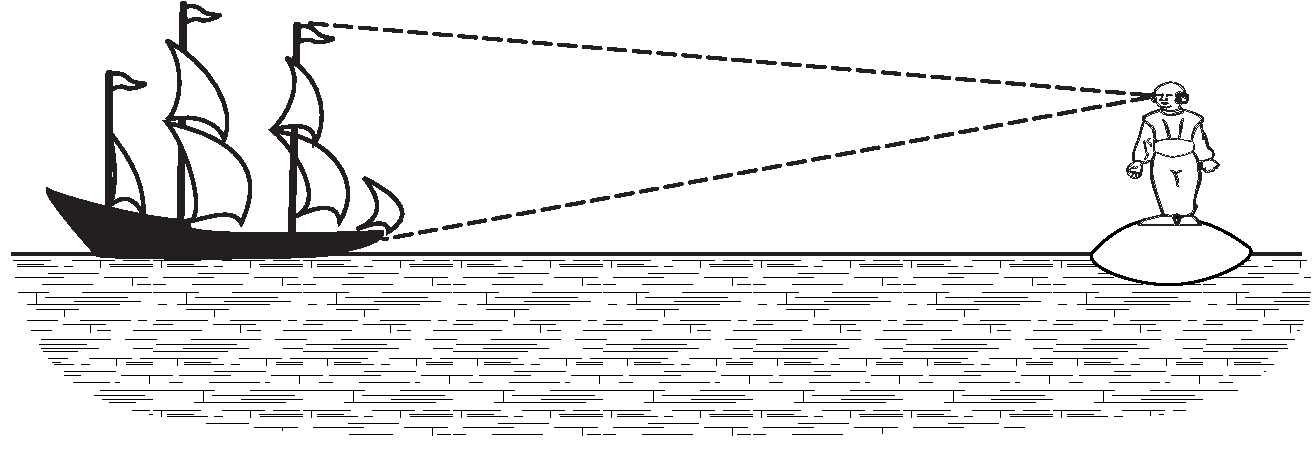
\includegraphics[width=.4\textwidth,page=1]{flatearth.pdf}}%
\hfill%
\textsf{b}~\parbox{.5\textwidth}{\includegraphics[width=.4\textwidth,page=2]{flatearth.pdf}}%



Our observations fit the second case, so Copernicus concludes that the Earth is round.

However, implicit in the argument is the assumption that light travels in a straight line. Suppose instead that light sags between the ship and the observer on the shore. When we see the mast and not the hull, perhaps the light is just sagging into the flat ocean; see figure c.

\medskip

\centerline{%
\textsf{c}~\parbox{.5\textwidth}{\includegraphics[width=.5\textwidth,page=3]{flatearth.pdf}}%
}

So, \emph{if} light travels in a straight line, \emph{then} our observation indicates that the Earth is round and figure b correctly illustrates what is going on. However, \emph{if} light sags, \emph{then} our observation indicates that the Earth is flat and figure c is correct.

At the outset of Copernicus' argument, we all just assumed that light travels in a straight line. But suppose you also thought, at the outset, that the Earth was flat. The argument relies upon the straight-line propagation of light to show that the Earth is round. Confronted with the argument and the observation, you might change your mind about the shape of the Earth. Alternately, you might change your mind about how light behaves. There is no rule of logic that tells you which change is the right one to make.

The same problem arises for scientists when an observation seems to conflict with some theory that they accept. Typically, the argument against the theory will require more premises than just the observation. It will also require other theoretical commitments--- like the belief in our example that light travels in a straight line. The scientists may save their theory from refutation by abandoning the other commitments.

This point was made famous by WVO Quine in the essay `Two Dogmas of Empiricism', where he attributed it to Pierre Duhem. So it is often called the \emph{Duhem-Quine problem}. 

The natural response, in our example, is to insist that optics is pretty well established. The assumption that light travels in a straight line through a uniform medium makes sense of lots of different phenomena. There would be serious consequences elsewhere in our system of belief if we were to start thinking that light sags, so we accept the consequence that the Earth is round. To use Duhem's phrase, our \emph{good sense} leads us to resolves the matter one way rather than the other. He insists, however, that good sense is not a precise logical rule.

\newbit You might wonder, though, why there couldn't be a precise logical rule to handle examples like the one above.

%Ptolemy Almagest I.V


\subsection{The material theory of induction, again}

We saw that one resolution to the problem of induction was to rely on material postulates, background knowledge about particular kinds of things. We generalize about samples of pure gold, for example, because gold is an element which only really comes in one form. The assumption that light travels in a straight line is another material postulate.

One way of putting the Duhem-Quine problem is that it is always possible to call material postulates into question. Ampliative inference requires that we start with some knowledge about the aspects of the world that we are studying, but (at least in principle) what we think we know can turn out to be wrong.



\label{theend}
\end{document}

